\documentclass[a4paper,10pt]{article}
\usepackage[utf8]{inputenc}
\usepackage[english]{babel}
\usepackage[onehalfspacing]{setspace}
\usepackage{float}
\usepackage{biblatex}   % Using reference package
\addbibresource{mybibliography.bib}

\usepackage[nottoc]{tocbibind} %Adds "References" to the table of contents
\usepackage{graphicx}
\usepackage{hyperref}
%\graphicspath{/home/trung/Pictures/} \usepackage{float}
\hypersetup{
    colorlinks=true,
    linkcolor=blue,
    filecolor=magenta,      
    urlcolor=cyan,
}
%Document title, author and date (empty)
\title{Python Guideline for Beginner}
\author{Trung Nguyen}
\date{}

%Beginning of the document
\begin{document}

\maketitle

\tableofcontents

\section{Introduction}

Currently (March 2020) Python is one of the most popular programming languages. According to the PYPL PopularitY of Programming Language Index, a search for a tutorial looks for a Python tutorial in 31.17\% of the cases [\href{http://pypl.github.io/PYPL.html}{PYPL}] \cite{PYPL}.\newline
Python is a \emph{script} language, whereby each line of the script is read and executed by the  \emph{Python interpreter}. Python scripts may \emph{import} other Python scripts in the form of \emph {packages}. The collection of packages used in a Python program should fit together and constitutes a \emph{Python environment}. Buiding an environment and choosing the right versions of Python packages for a task is best left to a \emph{package manager}.\newline
Anaconda is a free and open-source tool for Python package management and \emph{deployment}. Anaconda is platform-independent and will help managing your Python libraries on Windows, Linux, and Mac OS. This means that it will handle module dependencies and provides you with a Python environment. The virtual environment manager allows you to install an independent development environment for each project. You can switch between environments like with other tools (\textit{e.g.} virtualenv).\\ 
This document will guide the starter on how to set up the environment from scratch, starting with the installation.
If you have already installed Anaconda, skip the Software Installation and start immediately by going to the \hyperref[sec:start]{Getting Started} section.


% ---------------------------------------------------------------------

\section{ Software Installation}

Installation of the Anaconda package manager can be done in two different ways:
\begin{itemize}
	\item installation of Miniconda, the console version. Download from \href{https://docs.conda.io/en/latest/miniconda.html}{Miniconda}
	\item installation of Anaconda Navigator, the GUI version. Download from \href{https://www.anaconda.com/products/individual}{Anaconda}.
\end{itemize}

In both cases, the package manager itself is named: \textbf{conda}.\\
This document covers the scope of installing the software on Linux. However, installation on Windows and MacOS is very similar (consult Google on how to install Miniconda or Anaconda Navigator for these operating systems).\\

For Miniconda, the console version, select the Linux installer (Python 3.x, 64-bit) and download. Install “Just for me” and a "$\sim$/Miniconda3" folder is created in your home directory.
Note: your username should NOT contain spaces.
Choose default options for all possible installer choices.

Once installed, open a terminal window and type: "conda -V" and see if the installation has been succesful. If so, you see the current version of the conda package manager and the (base) prompt, to indicate you are in the base environment, which you will, however, not use very often.\\

\begin{figure}[H]
	\centering
	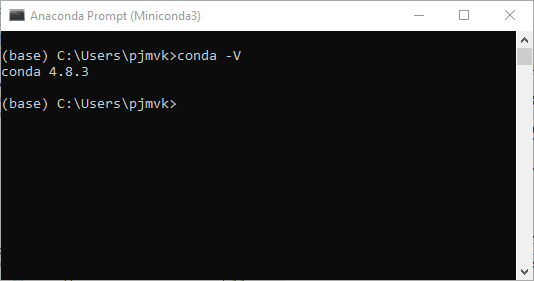
\includegraphics[width=0.8\columnwidth]{Pictures/Miniconda_prompt.png}
	\caption[Short title]{Miniconda}
	\label{fig:Miniconda}\end{figure}

For the installation of Anaconda Navigator (GUI), select the linux installer (Python 3.x, 64-bit) and download. The GUI is automatically installed when you install Anaconda version 4.0.0 or higher. Install “Just for me” and a  "$\sim$/Anaconda3" folder is created in your home directory.
Note: your username should NOT contain spaces.
Choose default options for all possible installer choices.

Note: If you have Miniconda or an older version of Anaconda installed, you can install Navigator from an Anaconda Prompt (console) by running the command:" conda install anaconda-navigator ".\\

The Anaconda Navigator user interface looks like the picture below:

\vspace{5mm}

\begin{figure}[H]
\centering
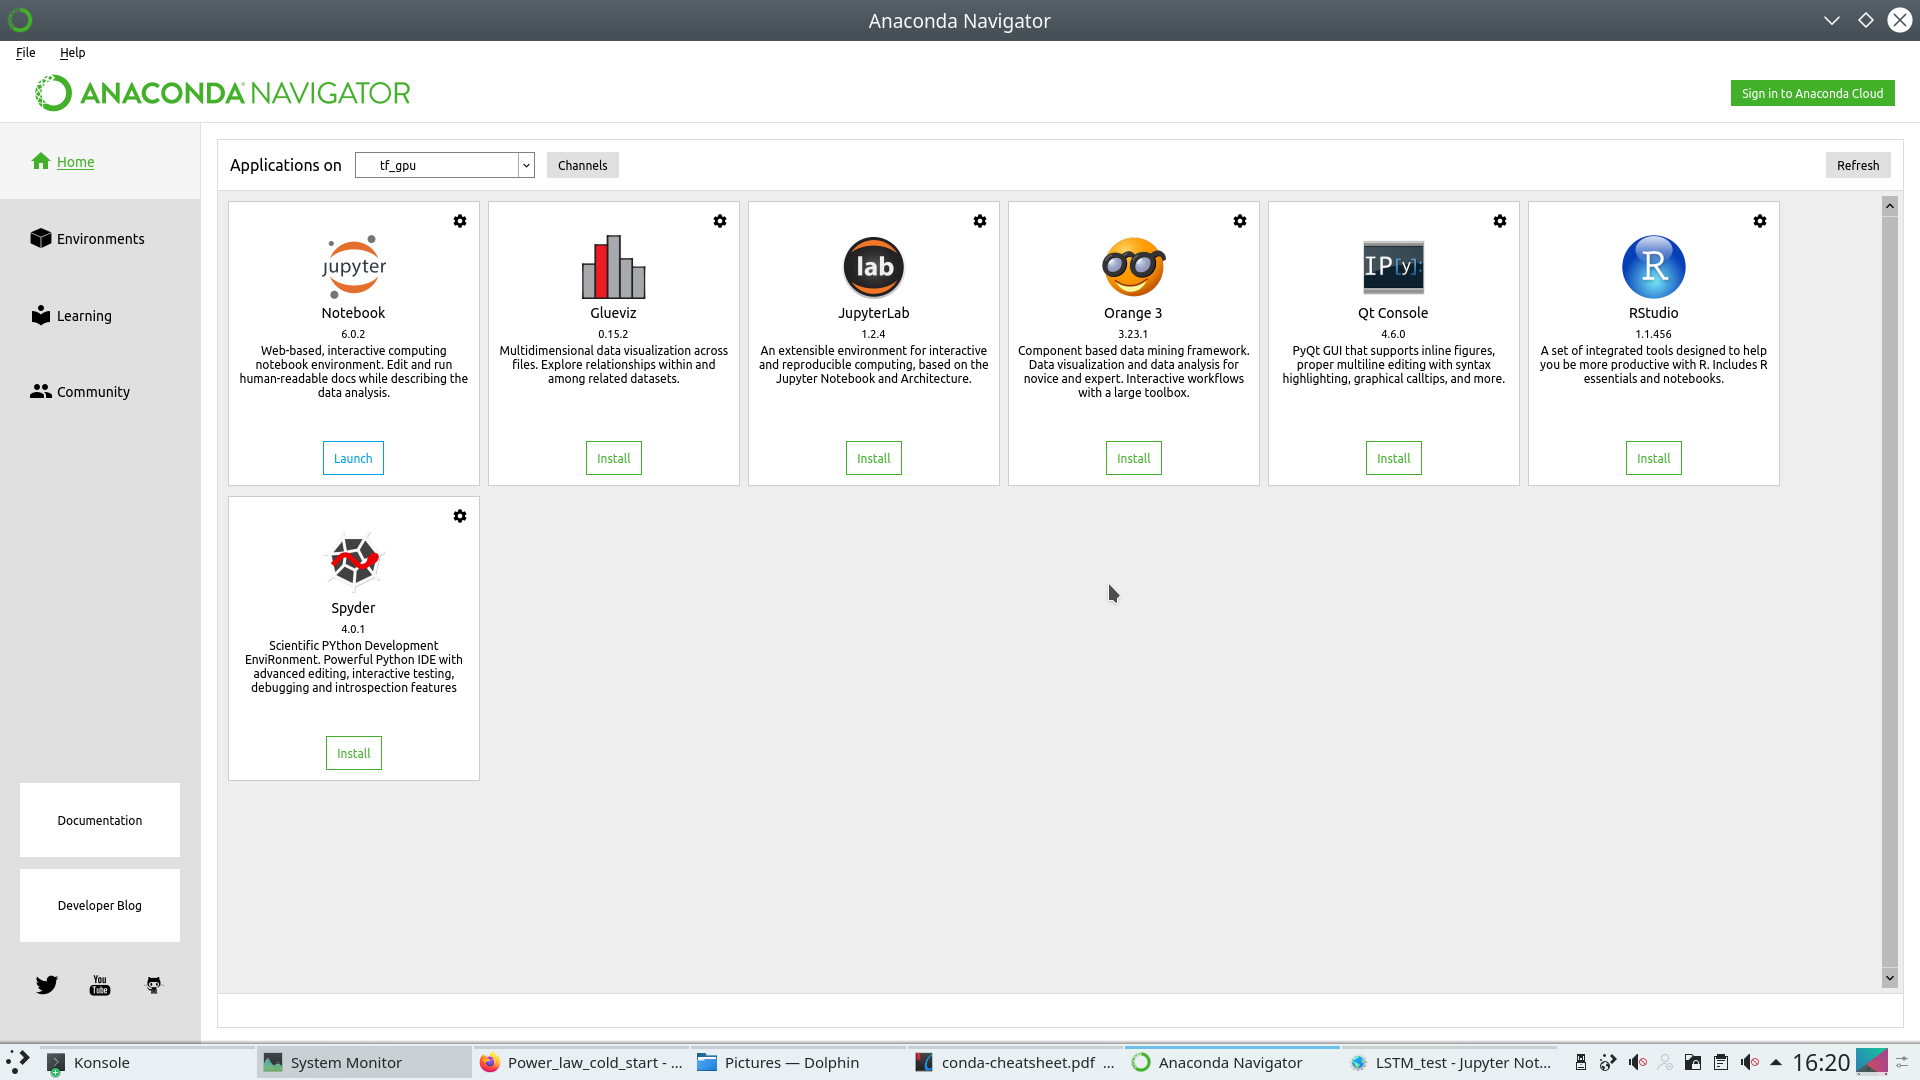
\includegraphics[width=1\columnwidth]{Pictures/Anaconda_navigator.png}
\caption[Short title]{Anaconda navigator}
\label{fig:Navigator}\end{figure}

\vspace{5mm}

\section{Environments}

The initial Miniconda installation comes with a single \textbf{base} environment, which is visible in the terminal prompt.

The command: \textbf{(base) $\left<pwd\right>$conda list} shows all installed packages in the \textbf{base} environment. $\left<pwd\right>$ stands for the present folder, included in the terminal prompt as usual.
Other \textbf{conda} commands can be given in the terminal to achieve full control over the Python environments and packages. A good practice is, to download a conda \emph{cheat-sheet} (Google with key word conda cheat sheet). In such a document, you can find how to \emph{create} a virtual environment and \emph{activate} it.\\
A new environment is created with:\\ 
\textbf{(base) $\left<pwd\right>$conda create –n $\left<env\_name\right>$ python=3.x}.\\ 
This creates an environment with the basic packages.

An important step is that you have to move to your new environment with:
\textbf{(base) $\left<pwd\right>$activate $\left<env\_name\right>$}.\\  
This changes the prompt into:\\
\textbf{(new\_name) $\left<pwd\right>$activate $\left<env\_name\right>$}.\\
and thus signals you the transfer to your newly created environment.
Type \textbf{conda list} to see the basic packages of your new environment.\\

An alternative option is using the Anaconda Navigator graphical user interface.
The folllowing link provides information on environments in Anaconda and the purpose of using them:
\href{https://protostar.space/why-you-need-python-environments-and-how-to-manage-them-with-conda}{Environments}.\\

The Anaconda "Environments" window is shown in Figure~\ref{fig:Anaconda_environment}. Have a look at the packages installed in the base environment. Create a new environment with the "Create" button in the lower left of the window. Have a look at the packages installed in your new environment.
These steps are identical to the steps executed in Miniconda: under the hood, the GUI types and carries out the terminal commands for you!

\begin{figure}[H]
\centering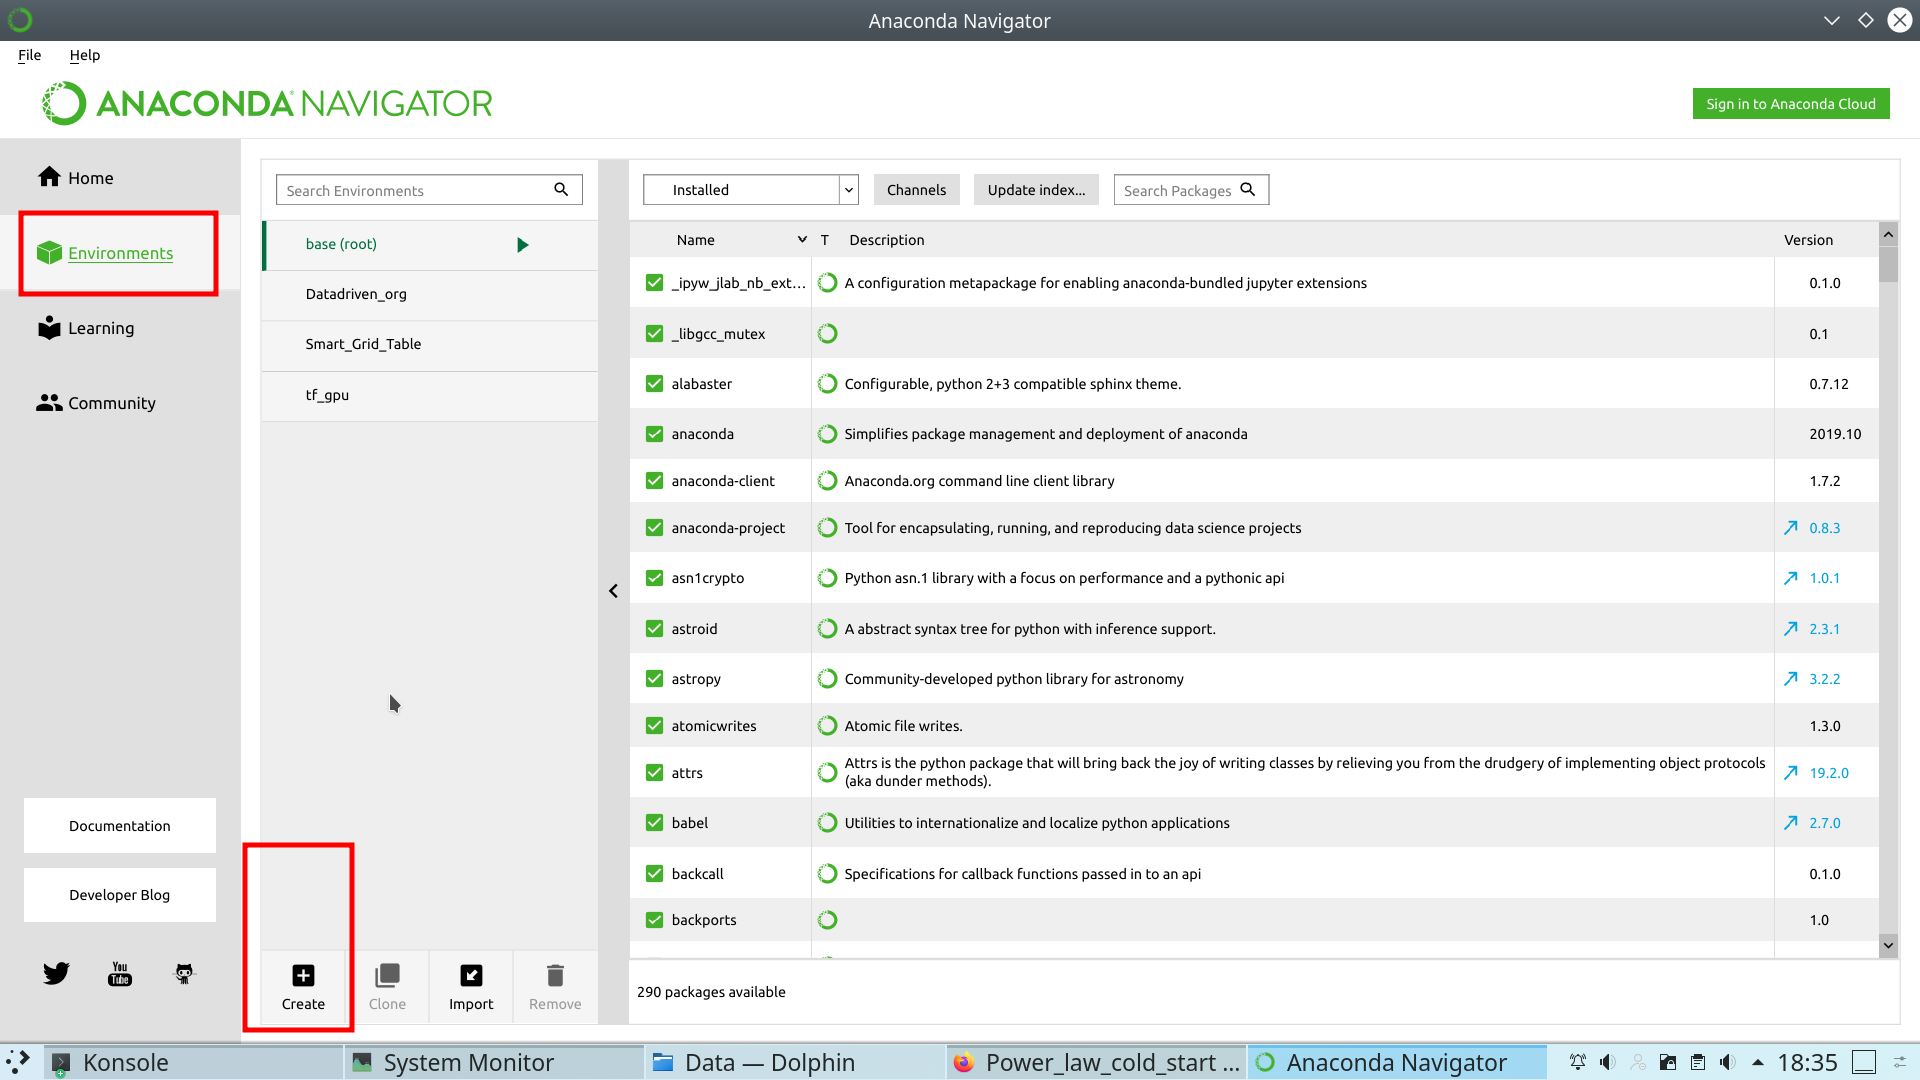
\includegraphics[width=1\columnwidth]{Pictures/env.png}
\caption[Short title]{create environment}
\label{fig:Anaconda_environment}\end{figure}


In general, upon creating a new environment, a few (Miniconda) or quite a lot (Anaconda Navigator) standard packages will be installed in the new environment. However, in both cases most of the useful packages (libraries) need to be installed manually.\\   
There are multiple ways to install the missing packages.Search for the missing packages and install with anaconda-navigator. Look at instruction on pictures below:

\vspace{5mm}
\begin{figure}[H]
\centering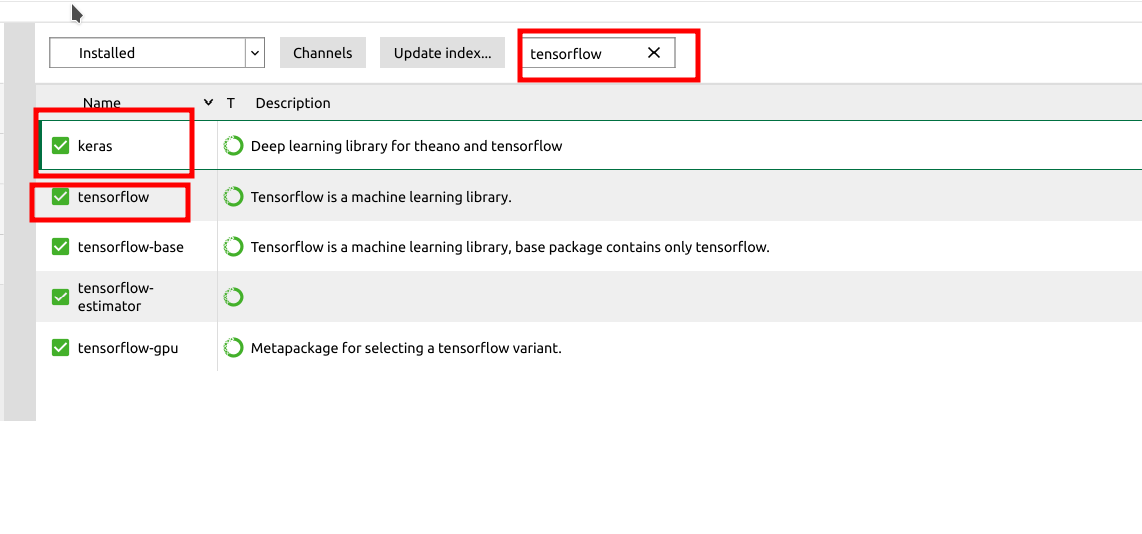
\includegraphics[width=1\columnwidth]{Pictures/packages.png}
\caption[Short title]{install packages}
\label{fig:ff3}\end{figure}

Installing packages with Console. Keep in mind that the virtual environment needs to be \emph{activated} before installing the missing packages.

\begin{figure}[H]
\centering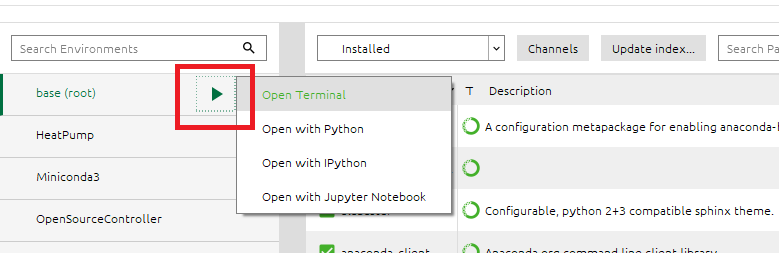
\includegraphics[width=1\columnwidth]{Pictures/Open_terminal.png}
\caption[Short title]{Open terminal}
\label{fig:ff4}\end{figure}

\begin{figure}[H]
\centering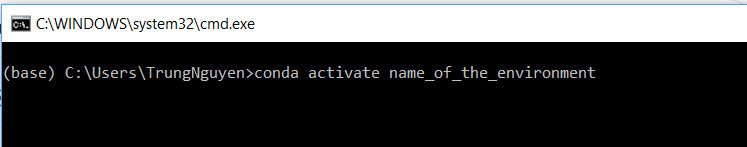
\includegraphics[width=1\columnwidth]{Pictures/activate_env.png}
\caption[Short title]{Activate Environment}
\label{fig:ff5}\end{figure}

Find the missing packages from :\href{https://anaconda.org/conda-forge/repo}{Anaconda repo}.\\ 
Copy one of the command in the red box and paste to the terminal.

\begin{figure}[H]
\centering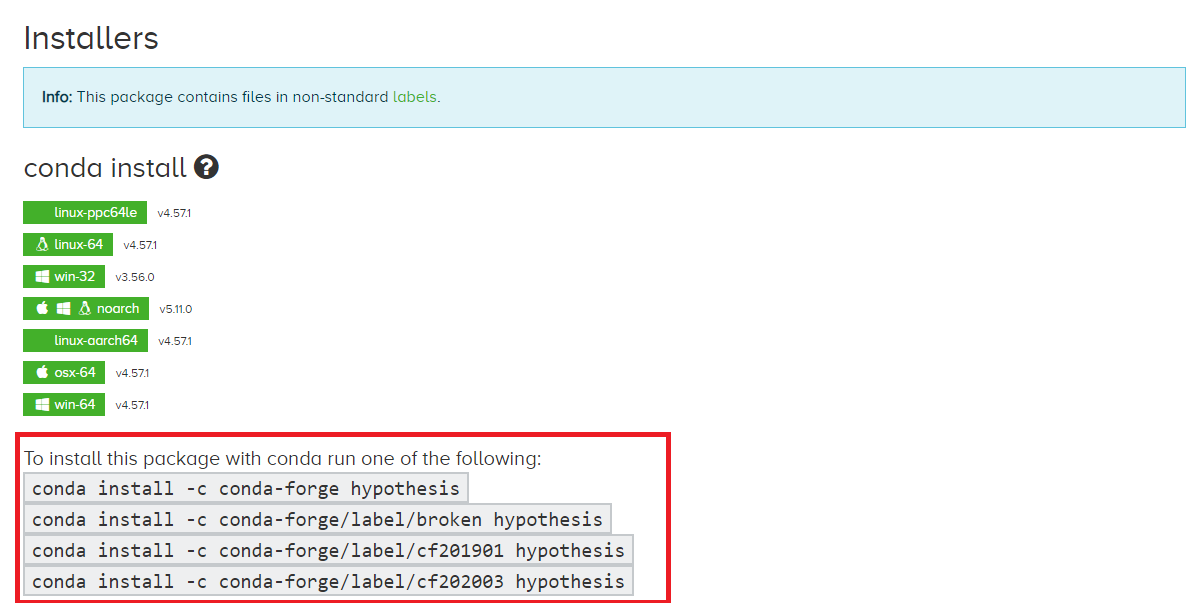
\includegraphics[width=1\columnwidth]{Pictures/install_pack.png}
\caption[Short title]{Install package}
\label{fig:ff6}\end{figure}

For some users, Miniconda will seem a more obvious option for installing new packages in an environment. The \textbf{activate} and \textbf{conda install -c $\left<channel\right>$ 
	$\left<package\right>$} commands can just be entered in the terminal window.\\

\textit{Note on using environments:}
It is customary to create a tailor-made environment for each Python project. Therefore, the information on installed packages needs to be shared among the project contributors. We'll see later in this document how that is done.


\medskip

% ---------------------------------------------------------------------

\section{Getting started}
\label{sec:start}

Now you can install Jupyter Notebook and Sypder for working with Python.\\
The easiest way to get start is using a Jupyter notebook.
"The Jupyter Notebook is an open-source web application that allows you to create and share documents that contain live code, equations, visualizations and narrative text. Uses include: data cleaning and transformation, numerical simulation, statistical modeling, data visualization, machine learning, and much more." \cite{Jupyternotebook}.\\
There are several alternative online Jupyter note book available for free such as \href{https://colab.research.google.com/notebooks/welcome.ipynb}{Google Colab},\href{https://www.kaggle.com/}{Kaggle},...etc. The instruction on how to setup these online platform will be discusses in separate document.\\
Open Jupyter note book by click "Launch"

\begin{figure}[H]
\centering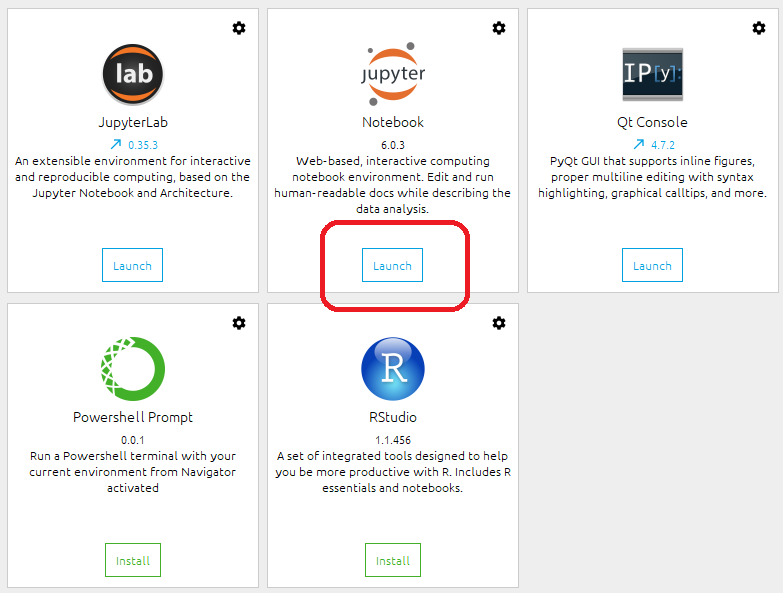
\includegraphics[width=1\columnwidth]{Pictures/Jupyter.png}
\caption[Short title]{Open Jupyter notebook}
\label{fig:ff7}\end{figure}

\begin{figure}[H]
\centering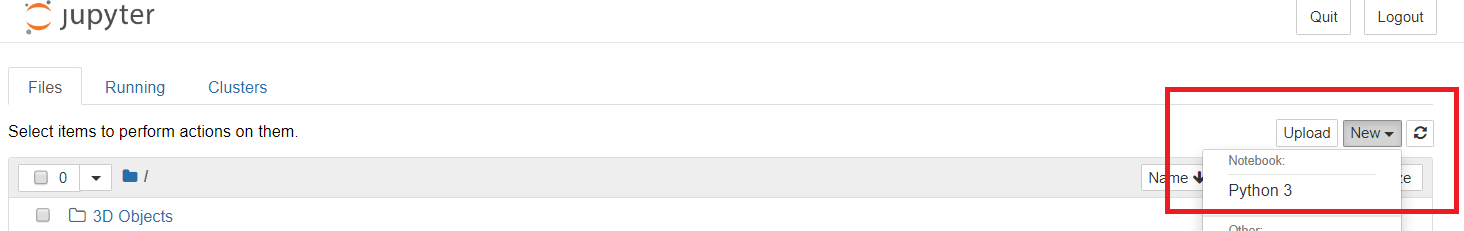
\includegraphics[width=1\columnwidth]{Pictures/Jupyter_new.png}
\caption[Short title]{Create a new python 3 project}
\label{fig:ff8}\end{figure}

\vspace{1cm}

Now try to write something with Jupyter notebook and click Run button or "Shift-Enter"

\begin{figure}[H]
\centering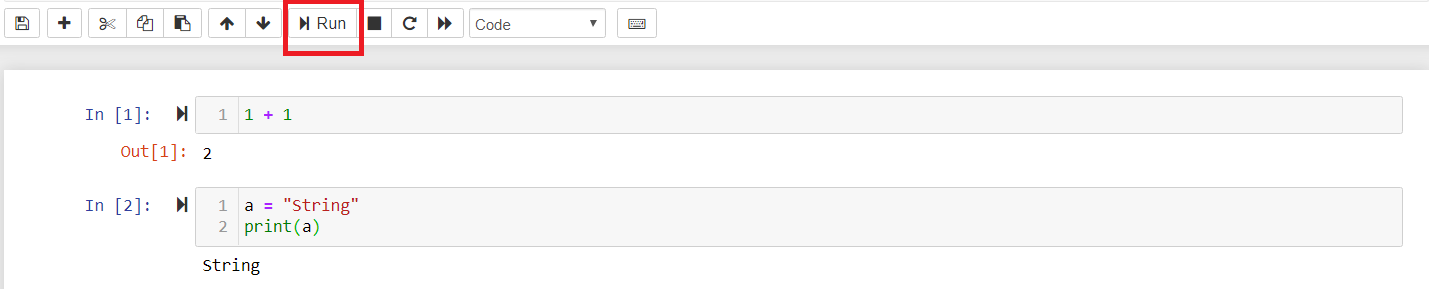
\includegraphics[width=1\columnwidth]{Pictures/Jupyter_try.png}
\caption[Short title]{Simple example}
\label{fig:ff9}\end{figure}

\vspace{1cm}

Downloading \href{https://nbviewer.jupyter.org/github/jupyter/notebook/blob/master/docs/source/examples/Notebook/Running\%20Code.ipynb#}{Notebook example}. Click execute on Binder to try it online on your browser


\begin{figure}[H]
\centering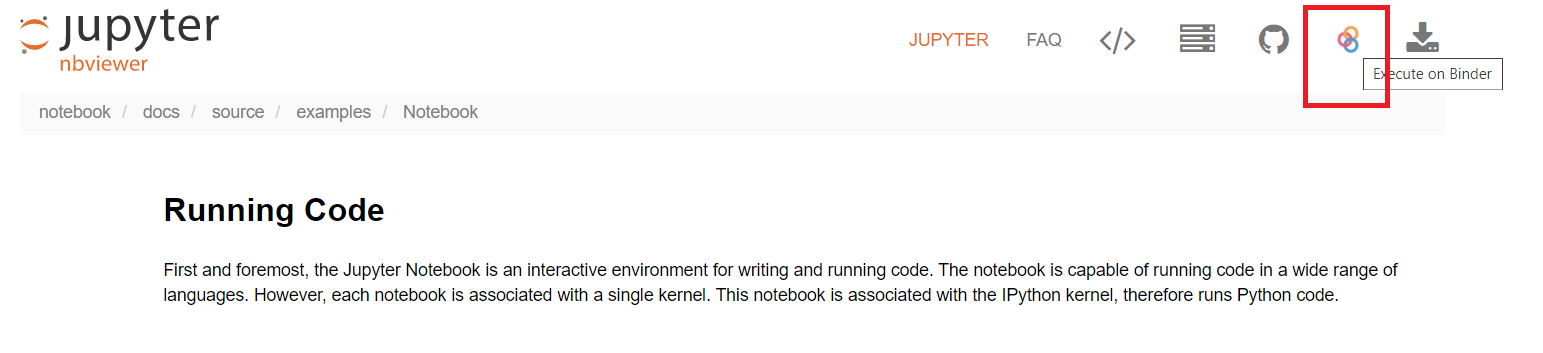
\includegraphics[width=1\columnwidth]{Pictures/Jupyter_online_try.png}
\caption[Short title]{Online example}
\label{fig:ff10}\end{figure}

\vspace{1cm}

\href{https://github.com/jupyter/notebook/blob/master/docs/source/examples/Notebook/Running\%20Code.ipynb}{Github example folder}.\\
Using google search with key world "Jupyter notebook for beginner"

%---------------------------------------------------------

\section{Link to relevant information}

\hspace{3ex}\href{https://docs.anaconda.com/anaconda/user-guide/cheatsheet/}{Anaconda user guide cheatsheet}.

\href{https://docs.anaconda.com/anaconda/navigator/}{Navigator docs}


%-------------------------------------------------------------------------

\section{List of Documentation}

\begin{enumerate}
  \item Python Guideline for Beginner.
  \item Setting up Online Python Notebook
  \item update...
\end{enumerate}

\vspace{1cm}
\vspace{1cm}




%----------------------------------------------------------------

\section{Recommendation Courses}

\href{https://www.coursera.org/learn/machine-learning}{Machine learning by Andrew Ng.}\\
\href{https://www.usfca.edu/data-institute/certificates/deep-learning-part-one}{Deep Learning using FastAI  by Jeremy Howard.}


%----------------------------------------------------------------


%Bibliographic references
\printbibliography

\end{document}
